\documentclass[sigconf]{acmart}

\usepackage[textsize=footnotesize]{todonotes}
\presetkeys{todonotes}{fancyline}{}

\usepackage{acronym}
\acrodef{DCAP}{Data Center Attestation Primitives}
\acrodef{DHKE}{Diffie-Hellman Key Exchange}
\acrodef{DMA}{Direct Memory Access}
\acrodef{ECU}{Electronic Control Unit}
\acrodef{EDL}{Enclave Definition Language}
\acrodef{EDP}{Enclave Development Platform}
\acrodef{EPID}{Enhanced Privacy ID}
\acrodef{GCM}{Galois-Counter Mode}
\acrodef{HUK}{Hardware Unique Key}
\acrodef{JWT}{JSON Web Token}
\acrodef{IAS}{Intel Attestation Server}
\acrodef{KDF}{Key Derivation Function}
\acrodef{LOC}{line of code}
\acrodefplural{LOC}[LOCs]{lines of code}
\acrodef{MAC}{Message Authentication Code}
\acrodef{MMIO}{Memory-Mapped I/O}
\acrodef{PCBAC}{Program Counter Based Access Control}
\acrodef{PCCS}{Provisioning Certificate Caching Service}
\acrodef{PCS}{Provisioning Certification Service}
\acrodef{PKI}{Public Key Infrastructure}
\acrodef{PSK}{Pre-Shared Key}
\acrodef{PTA}{Pseudo Trusted Application}
\acrodef{QE}{Quoting Enclave}
\acrodef{RTT}{round-trip time}
\acrodef{SDK}{Software Development Kit}
\acrodef{SEV}{Secure Encrypted Virtualization}
\acrodef{SGX}{Software Guard Extensions}
\acrodef{SM}{Software Module}
\acrodef{TCB}{Trusted Computing Base}
\acrodef{TEE}{Trusted Execution Environment}
\acrodef{V2X}{Vehicle-to-Everything}
\acrodef{WSN}{Wireless Sensor Network}


\fancyhf{} % Remove fancy page headers 
\fancyhead[C]{Submission \#pp012 to ACM CCS 2021}
\fancyfoot[C]{\thepage}

\settopmatter{printacmref=true}
%\settopmatter{printacmref=true, printccs=true, printfolios=true}

\copyrightyear{2021}
\acmYear{2021}
\setcopyright{rightsretained}
\acmConference[CCS '21]{Proceedings of the 2021 ACM SIGSAC Conference on Computer and Communications Security}{November 15--19, 2021}{Virtual Event, Republic of Korea}
\acmBooktitle{Proceedings of the 2021 ACM SIGSAC Conference on Computer and Communications Security (CCS '21), November 15--19, 2021, Virtual Event, Republic of Korea}\acmDOI{10.1145/3460120.3485341}
\acmISBN{978-1-4503-8454-4/21/11}


\begin{document}
\fancyhead{}

\title{POSTER: An Open-Source Framework for Developing Heterogeneous
  Distributed Enclave Applications}

\author{Gianluca Scopelliti}
\email{gianluca.scopelliti@ericsson.com}
\affiliation{%
  \institution{imec-DistriNet, KU Leuven}
  \city{Leuven}
  \country{Belgium}
  \postcode{3001}
}
\author{Sepideh Pouyanrad}
\email{sepideh.pouyanrad@kuleuven.be}
\affiliation{%
  \institution{imec-DistriNet, KU Leuven}
  \city{Leuven}
  \country{Belgium}
  \postcode{3001}
}
\author{Job Noorman}
\email{job.noorman@kuleuven.be}
\affiliation{%
  \institution{imec-DistriNet, KU Leuven}
  \city{Leuven}
  \country{Belgium}
  \postcode{3001}
}
\author{Fritz Alder}
\email{fritz.alder@acm.org}
\affiliation{%
  \institution{imec-DistriNet, KU Leuven}
  \city{Leuven}
  \country{Belgium}
  \postcode{3001}
}
\author{Frank Piessens}
\email{frank.piessens@kuleuven.be}
\affiliation{%
  \institution{imec-DistriNet, KU Leuven}
  \city{Leuven}
  \country{Belgium}
  \postcode{3001}
}
\author{Jan Tobias M\"{u}hlberg}
\email{jantobias.muehlberg@kuleuven.be}
\affiliation{%
  \institution{imec-DistriNet, KU Leuven}
  \city{Leuven}
  \country{Belgium}
  \postcode{3001}
}

\begin{abstract}
%
We present an integrated open-source framework to develop, deploy, and use
event-driven distributed enclaved applications across heterogeneous Trusted
Execution Environments (TEEs). Our framework strives for strong application
authenticity and integrity guarantees, and optionally confidentiality and
availability, while minimizing the run-time Trusted Computing Base (TCB). For
software developers, our framework provides a high level of abstraction
over the platform-specific TEE layer that provides isolation, attestation
and secure communication amongst distributed application components,
allowing developers to focus of application logic. We provide a notion of
event-driven programming to develop distributed enclave applications in
Rust and C for heterogeneous TEEs, including Intel SGX, ARM TrustZone and
the open-source Sancus. This heterogeneity makes our framework uniquely
suitable for a broad range of use cases which combine cloud processing,
mobile and edge devices, and lightweight sensing and actuation.
%
\end{abstract}

\keywords{Trusted Execution; Event-Driven Systems; Intel SGX; ARM
TrustZone; Sancus}


% TODO: replace this section with code generated by the tool at https://dl.acm.org/ccs.cfm
\begin{CCSXML}
<ccs2012>
<concept>
<concept_id>10002978.10003006.10003007.10003009</concept_id>
<concept_desc>Security and privacy~Trusted computing</concept_desc>
<concept_significance>500</concept_significance>
</concept>
<concept>
<concept_id>10010520.10010553.10010559</concept_id>
<concept_desc>Computer systems organization~Sensors and actuators</concept_desc>
<concept_significance>500</concept_significance>
</concept>
<concept>
<concept_id>10010520.10010575.10010578</concept_id>
<concept_desc>Computer systems organization~Availability</concept_desc>
<concept_significance>300</concept_significance>
</concept>
<concept>
<concept_id>10010520.10010575.10010579</concept_id>
<concept_desc>Computer systems organization~Maintainability and maintenance</concept_desc>
<concept_significance>300</concept_significance>
</concept>
<concept>
<concept_id>10002978.10003006.10003013</concept_id>
<concept_desc>Security and privacy~Distributed systems security</concept_desc>
<concept_significance>500</concept_significance>
</concept>
</ccs2012>
\end{CCSXML}

\ccsdesc[500]{Security and privacy~Trusted computing}
\ccsdesc[500]{Security and privacy~Distributed systems security}
\ccsdesc[500]{Computer systems organization~Sensors and actuators}
\ccsdesc[300]{Computer systems organization~Availability}
\ccsdesc[300]{Computer systems organization~Maintainability and maintenance}
% -- end of section to replace with generated code




\maketitle
\renewcommand{\shortauthors}{Scopelliti and Pouyanrad et al.}
%
%\todo{need a name for the thing.}

% Authors are asked to submit a short proposal that describes the main
% contributions of the poster or demonstration. Proposals should contain a
% brief abstract, place an emphasis on the motivation for the work, and
% summarize contributions being presented. Preliminary results may also be
% included. The proposal should clearly state the difference of the work
% that will be presented with any paper published or under submission on
% the same topic. Presentation proposals will be evaluated primarily on
% their potential to stimulate interesting discussions, facilitate the
% exchange of ideas, and promote collaborations. Authors of accepted poster
% proposals will be provided instructions for preparing the posters. Poster
% session will be following the format of the main CCS conference (as
% announced here: ACM CCS 2021 - November 15-19, 2021 (sigsac.org)).
% Questions shall be directed via email to the Poster/Demo Chair.

\section{Introduction \& Problem}

\acp{TEE} allow an application to execute in a hardware-protected
environment called \emph{enclave}. Enclaves are isolated and protected from
the rest of the system, ensuring strong confidentiality and integrity
guarantees. Cryptographic primitives and cryptographic keys, which are unique per enclave
and which can only be used by that enclave, enable secure communication
and remote attestation; the latter is a mechanism to obtain cryptographic
proof that an application is running under enclave protection on a specific
processor.
%
There are several \acp{TEE} available, both in industry and research.
Open-source \acp{TEE} include Sancus and Keystone; proprietary options are,
e.g., SGX for Intel processors, SEV for AMD, TrustZone for ARM, and
others~\cite{maene:hardware}. Developing distributed applications that
execute on heterogeneous \acp{TEE} is difficult, in particular for
scenarios that combine Internet-of-Things, Edge, and cloud hardware: each
\ac{TEE} requires a platform-specific software implementation, comes with
different approaches to key management and attestation, a different
\ac{TCB} footprint, and provides slightly different hardware features and
security guarantees.
 
Therefore, developing a distributed application that uses a multitude of
\ac{TEE} architectures is non-trivial. A developer needs to make choices
as to which security features are required for which components, adapt the
code of each component to multiple specific platforms, arrange for different
deployment and attestation strategies, and implement secure interaction
between the components. Open-source projects such as Open Enclave SDK and
Google Asylo aim to bridge the development gap between different \acp{TEE}.
However, software engineers still need to account for the communication
between different modules, which has to be properly secured with
cryptographic operations for data encryption and authentication.  In
particular, the responsibility for deploying the distributed application,
loading and attesting each enclave, establishing session keys and secure
connections between distributed components, is still left to the
application developer and operator. Overall, ensuring strong security guarantees in
distributed scenarios poses a challenge to  the adoption of \ac{TEE}
technology.
%
\begin{figure*}[ht!]
%
  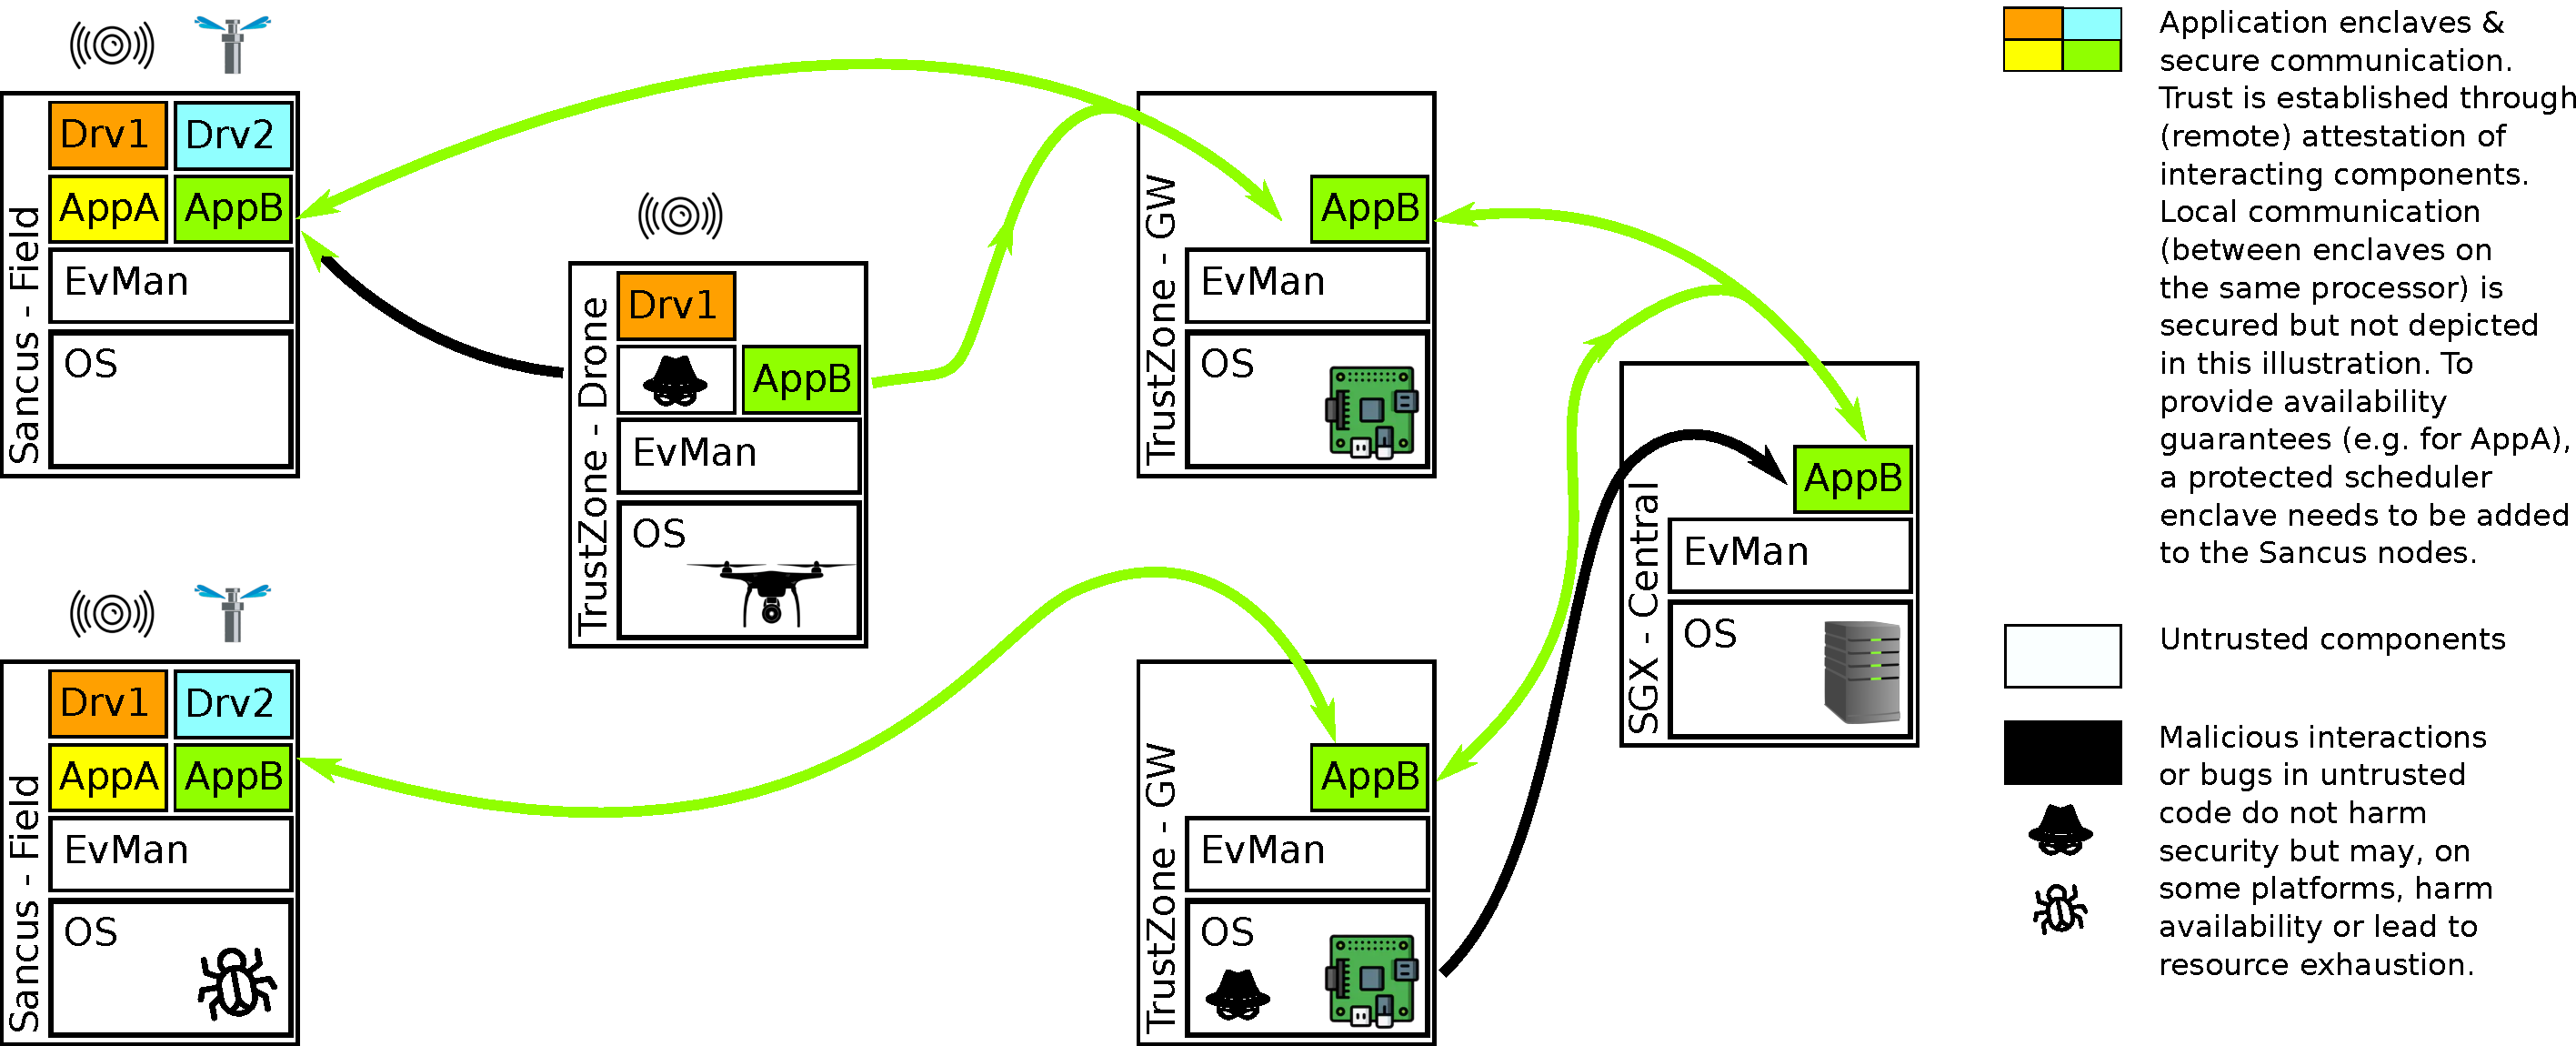
\includegraphics[height=55mm]{graphics/20210808-scenario.pdf}
%
  \caption{A smart irrigation system as an example for distributed
application networks we support. Light-weight sensing and actuation nodes
are deployed in a field. Application \emph{AppA} controls irrigation units
(through driver \emph{Drv2}) based on soil moisture (obtained through
\emph{Drv1}). Application \emph{AppB} provides the same functionality but
has access to additional data sources, e.g., aerial surveillance and data
aggregation on central infrastructure. All application components execute
in enclaves (colored).
% and are attested, and all communication between application components is
% at least authenticated and integrity protected.
Directed data flows through untrusted networks (colored arrows) are at
least  authenticated and integrity protected; attestation precedes the
establishment of all data flows, and a notion of local attestation is used
to establish trust between enclaves on the same processor. All other
software in the scenario is untrusted regarding our security properties,
which leads to a very small run-time application \ac{TCB}. Guaranteeing
availability properties may require a different compartmentalization
strategy. The concept is also applicable across, e.g., the different
control units within a car or in an autonomous robot.}
%
  \label{fig:scenario}
%
\end{figure*}
%
To address these challenges, our framework makes the following
contributions:
%
\begin{itemize}
%
  \item We present an integrated approach for the authentic execution of
event-driven programs on heterogeneous distributed systems, under the
assumption that the execution infrastructure offers specific security
primitives -- \acp{TEE} with support for secure I/O
(cf.~\cite{noorman_sancus2}) and real-time processing
(cf.~\cite{alder_2021_aion});
%
  \item We integrate a technique for implementing support for secure I/O by
means of protected driver modules, and availability through \ac{TEE}
extensions, on small \ac{TEE}-microprocessors such as
Sancus~\cite{noorman_sancus2};
%
  \item We provide a revised open-source implementation of the approach for
Intel SGX, ARM TrustZone, and for Sancus, which supports software
development in Rust and C;
%
  \item We work towards an extensive evaluation of performance and security
aspects of that implementation. Preliminary results show that our framework
allows for the deployment of complex distributed software systems with a
very small run-time application \ac{TCB}.
%
\end{itemize}
%
Our framework is available under an open-source license at
\url{https://github.com/AuthenticExecution/env}.


\section{Authentic Execution}

We developed the concept of \emph{authentic
execution}~\cite{noorman:authentic-execution} to address the problem of
securely executing distributed applications on a shared infrastructure and
to also minimize the application's runtime \ac{TCB}. Authentic
execution provides a notion of security that we summarize as ``if the
application produces a physical output event (e.g., turns on an LED), then
there must have happened a sequence of physical input events such that that
sequence, when processed by the application (as specified in the high-level
source code), produces that output event,'' which is roughly equivalent to
the concept of \emph{robust safety} in later
literature~\cite{abate2019journey}. This guarantee relies on standard
\ac{TEE} security properties -- i.e., strong software isolation and
software attestation -- but also on a notion of \emph{secure I/O} where
physical I/O channels can be connected to an 
% application's I/O channels 
enclave
such that the application enclaves maintain exclusive access over
I/O peripherals.

Initially, our approach did not consider confidentiality and availability.
Yet, our \ac{TEE}-design~\cite{noorman_sancus2} and a series of case
studies in application domains such as smart electricity metering, smart
agriculture and secure vehicular communications~\cite{muehlber_smart_meter,
scopelliti2020thesis, vanbulck_2017vulcan} did consider and
provide confidentiality. Most recently, in~\cite{alder_2021_aion}, we
address the availability aspect and extend light-weight embedded
\ac{TEE} architectures so as to provide strong temporal isolation
guarantees to multiple, mutually distrusting applications. To discuss the
interplay of these different concepts, we introduce an irrigation system as
a use case.

\subsection{Use Case: Automated Irrigation}

Smart farming applications are an essential part of modern critical
infrastructure. An automated irrigation system, as illustrated in
Figure~\ref{fig:scenario}, would involve a series of light-weight sensors
and actuators in the field that monitor soil moisture and control water supply
% ,e.g. by opening or closing valves on demand
. The system can be
connected to edge infrastructure or cloud services for centralized
configuration and maintenance, to integrate reporting and billing, and to
minimize water consumption based on weather predictions. Naturally, smart
farming systems are security critical since malicious interactions can
potentially lead to huge costs and may destroy a crop; they also demand a
high level of dependability where events must be guaranteed to be processed
in a timely manner. With our approach to building such applications as
event-driven systems, we intend to support developers with an intuitive
programming paradigm and automated enclave deployment to achieve the security objectives highlighted below.

\subsection{Security Objective}

We consider an \emph{open system} as the basis for our framework. In this
open system, software is deployed dynamically and multiple stakeholders may
run applications on the same infrastructure, including on the light-weight
IoT and Edge hardware. Thus, we consider scenarios where arbitrary new code
can be loaded at at run time and we consider powerful attackers that can
manipulate all the software on the infrastructure (unless that software is
isolated in enclaves), can manipulate network traffic, but cannot break
crypto. Attacks against the hardware are out of scope.

Under this attacker model, isolation and mutual attestation of all
application components, including peripheral driver, results in the initial
authenticity and integrity guarantees, where all observed outputs can be
explained in terms of a trace of (authentic) inputs and the (integrity
protected) source code of the application. Using the sealing capabilities
of \acp{TEE}, this guarantee can be extended to also provide
confidentiality of application events and state.
Our availability extensions
allow individual enclaves to execute with strong guarantees for
responsiveness and progress, which allows for these enclaves to timely
detect and react upon availability issues across the application.
We currently do not
consider protection from side-channel leakage as part of the framework but
as part of the developer's task to address. 

\subsection{Secure I/O}

Several \acp{TEE} such as ARM TrustZone and Sancus allow for I/O
peripherals to be exclusively controlled by the secure world or by an
enclave. In the case of Sancus, e.g., peripherals are controlled through
Memory-Mapped I/O. By mapping enclave memory over a peripheral's  memory
addresses, a driver enclave can gain exclusive control and manage access to
the peripheral. In our framework, these driver enclaves effectively
translate physical input and output channels into application events and
vice versa.  Secure I/O is essential for our security guarantee as it
prevents application inputs or outputs to be spoofed by software that is
not part of the attested application \ac{TCB}. Our framework provides a
notion of end-to-end security by seamlessly integrating application
enclaves on \acp{TEE} that provide secure I/O with \acp{TEE} that do not.

\subsection{Availability Guarantees}

In~\cite{alder_2021_aion}, we extend Sancus towards a configurable security
architecture that provides a notion of guaranteed real-time execution for
dynamically loaded enclaves.  We implement preemptive multitasking and
restricted atomicity on top of strong software isolation and software
attestation. Our approach enables the hardware to enforce confidentiality
and integrity protections while a decoupled small software component can
enforce availability and guarantee strict deadlines of a bounded number of
protected applications, without introducing a notion of priorities amongst
these applications. This allows us to develop enclaves that can handle
interrupts and make progress with deterministic activation latencies, even
in the presence of a strong adversary with arbitrary code execution
capabilities. In the context of our authentic execution framework, these
enclaves can serve as a means to implement dependable sensing and control
loops, but also to provide a reliable notion of time and progress across a
distributed application, and to
detect the lack of progress in such applications.

\subsection{Software Architecture \& Deployment}

Application code is developed using macros and annotations to define the
name and scope of enclaves, and to label input and output channels of each
application component. A \emph{deployment descriptor} specifies which
component is to be loaded on which target machine, and how the respective
input and output channels are to be linked together, and what
communications interfaces are being used. Component loading and
communication are facilitated by infrastructure software, which is
untrusted regarding our security properties but needs to be trusted
regarding availability. Our framework provides an enclave that facilitates
the initial attestation and key management steps during the automated
deployment phase. We build upon established software development tool
chains for the respective source languages and target architectures.

\section{Summary}

We presented an open-source framework for developing heterogeneous
distributed enclave applications with an event-driven programming model.
Our approach is distinguished by enabling an open-system approach where
distrusting stakeholders can share processing resources, by supporting a
range of \acp{TEE}, from the cloud to edge and IoT devices, and by
providing a unique set of security and availability guarantees that enable
advanced use cases, e.g., in safety-critical sensing and actuation.

\begin{acks}
%
This research is partially funded by the Research Fund KU Leuven, the
Flemish Research Programme Cybersecurity, and the SAFETEE project at KU
Leuven. This research has received funding under EU H2020 MSCA-ITN action
5GhOSTS, grant agreement no. 814035. Fritz Alder is supported by the
Research Foundation Flanders.
%
\end{acks}

\bibliographystyle{ACM-Reference-Format}
\bibliography{bibliography.bib}

\end{document}
